\sep
\section{Zufallsvariablen und Verteilungsfunktionen}
\subsection{Abstrakte Definition }
\Def[2.1 Zufallsvariable] \newline
Sei \( (\omega, \mathcal{F}, \mathbb{P})\) ein Wahrscheinlichkeitsraum. Eine Zufallsvariable ist eine Abbildung \( X : \omega \rightarrow \mathbb{R} \) so dass, für alle \( a \in \mathbb{R}\) gilt \[ \{ w \in \omega : X(w) \leq a \} \in \mathcal{F}\]
\Bem  \newline
Für Ereignisse im Bezug auf Z:V
\begin{itemize}
    \item \( \{X \leq a \} = \{ w \in \omega : X(w) \leq a\}\)
    \item \( \{ a < X \leq b \} = \{ w \in \omega : a < X(w) < b\}\)
    \item \( \{ X \in \mathbb{Z}\} = \{ w \in \omega : X(w) \in \mathbb{Z}\}\)
\end{itemize}
\[ \mathbb{P}[X \leq a] = \mathbb{P}[\{X \leq a\}] = \mathbb{P}[\{w \in \omega : X(w) \leq a\}]\]
\subsection{Verteilungsfunktion}
\Def[2.2 Verteilungsfunktion] \newline
Sei X eine Zufallsvariable auf einem W-Raum \( (\omega, \mathcal{F}, \mathbb{P})\). Die Verteilungsfunktion von X ist eine Funtkion \(F_X : \mathbb{R} \rightarrow [0,1]\), definiert durch \[ \forall a \in \mathbb{R} \ F_X(a) = \mathbb{P}[X \leq a]\]
\Satz[2.3 Einfache Identität] \newline
Seien \(a < b\) zwei reelle Zahlen. Dann gilt \[ \mathbb{P}[a < X \leq b ] = F(b) - F(a)\]
\Theo[2.4 Eigenschaften der Verteilungsfunktion] \newline
Sei X eine Z.V aif einem Wahrscheinlichkeitsraum. Die Verteilungsfunktion \( F = F_X : \R \rightarrow [0,1]\) von X erfüllt folgende Eigenschaften
\begin{itemize}
    \item F ist monoton wachsend
    \item F ist rechtsstetig
    \item \( \lim_{a \rightarrow -\infty} F(a) = 0 \) und \( \lim_{a \rightarrow \infty} F(a) = 1\)
\end{itemize}
\subsection{Unabhängigkeit von Zufallsvariablen}
\Def[2.5] \newline
Seien \( X_1 \dots X_n \) Zufallsvariablen auf einem W-Raum. Dann heissen \(X_1, \dots X_n \) unabhängig falls \[ \forall x_1, x_2 \dots x_n \in \R \] \[\mathbb{P}[X_1 \leq x_1 \dots X_n \leq x_n ] = \mathbb{P}[X_1 \leq x_1] \dots \mathbb{P}[X_n \leq x_n]\]
\Satz[2.7 Gruppieren von Zufallsvariablen] \newline
Seien \(X_1 \dots X_n\) n unabhängige Zufallsvariablen. Seien \( 1 \leq i_1 < i_2 < \dots < i_k \leq n \) Indizes und \(\phi_1 \dots \phi_k\) Abbildungen. Dann sind  \[ Y_1 = \phi_1(X_1 \dots X_{i_1}), Y_2 = \phi_2(X_{i_{1}+1}, \dots X_{i_2}), \dots \] \[Y_k = \phi_k(X_{i_{k-1}+1} \dots X_{i_k})\] unabhängig \newline
\newline \newline
\Def[2.8] \newline
Eine Folge von Zufallsvariablen \(X_1, X_2, \dots \) heisst
\begin{itemize}
    \item unabhängig falls \(X_1, \dots X_n \) unabhängig sind, für alle \(n \in  \N\)
    \item unabhängig und identisch verteilt(uiv) falls sie unabhängig ist und die Zufallsvariablen dieselbe Verteilungsfunktion haben d.h \[ \forall i, j \ F_{X_i} = F_{X_j}\]
\end{itemize}
\subsection{Konstruktion von Zufallsvariablen}
\Def[2.9] \newline
Sei \(p \in [0,1]\). Eine Zufallsvariable X heisst Bernoulli ZUfallsvariable mit Parameter p falls \[\mathbb{P}[X=0] = 1 - p \ \text{und} \ \mathbb{P}[X=1] = p\]
Dabei schreiben wir \( X \sim Ber(p)\)
\Theo[2.10 Existenzsatz von Kolmogorov] \newline
Es existiert ein W-Raum \( (\Omega, \mathcal{F}, \mathbb{P}) \) und eine nicht endliche uiv Folge von Bernoulli Zufallsvariablen \(X_1, X_2, \dots \) auf \( (\Omega, \mathcal{F}, \mathbb{P}) \) mit Paramter \(\frac{1}{2}\)
\Def[2.11] \newline
Eine Zufallsvariable U heisst gleichverteilt auf \([0,1]\) falls ihre Verteilungsfunktion gegeben ist durch\[F_U(x) = \left.
    \begin{cases}
    0 & x < 0 \\
    x & 0 \leq x \leq 1 \\
    1 &  x > 1
\end{cases}
\right.\]
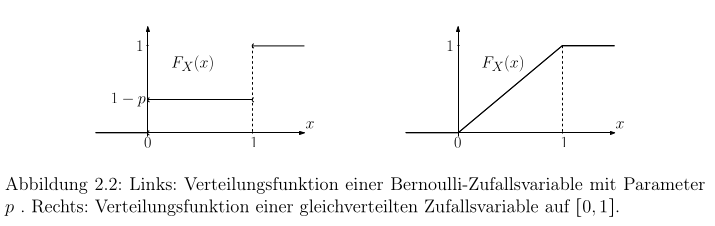
\includegraphics[scale=0.3]{abb2.2.png}
\Def[2.13 Pseudoinverse] \newline
Die Pseudoinverse von F ist eine Abbildung \(F^{-1} : (0,1) \rightarrow \R \) definiert durch \[ \forall \alpha \in (0,1) \ F^{-1} = \inf{x \in \R : F(x) \geq \alpha}\]
Nach Definition des Infimums und unter Verwendung der rechten Stetigkeit von F ergibt sich für jedes \(x \in \R \) und \( \alpha \in (0,1)\)
\[ (F^{-1}(\alpha) \leq x ) \Leftrightarrow (\alpha \leq F(x))\]
\Theo[2.14 Inversionsmethode] \newline
Sei \(F: \rightarrow [0,1]\) eine Abbildung, welche Eigenschaften 1-3 erfüllt. Sei U eine Gleichverteilte Zufallsvariable. Dann besitzt die Zufallsvariable
\[X = F^{-1}(U)\]
gerade die Verteilungsfunktion \(F_X = F\)
